\documentclass[t,10pt,aspectratio=169]{beamer}
%\usetheme{Berkeley}
\usepackage{graphicx}
\usepackage{amsmath}
\usepackage[american]{circuitikz}
\usepackage{tcolorbox}


\title{Clase 24}
\subtitle{El transistor MOSFET no ideal I}
\author{Dr.-Ing. Juan José Montero Rodríguez}
\subject{Elementos Activos}
\institute{Escuela de Ingeniería Electrónica}
\date{Semestre II-2023}
\titlegraphic{
\includegraphics[height=8mm]{./figuras/logotec.pdf}}


\begin{document}

\begin{frame}{}
\maketitle
\end{frame}


\section{Modulación de canal}
\begin{frame}{Modulación de longitud de canal}

\begin{figure}[H]
    \centering
    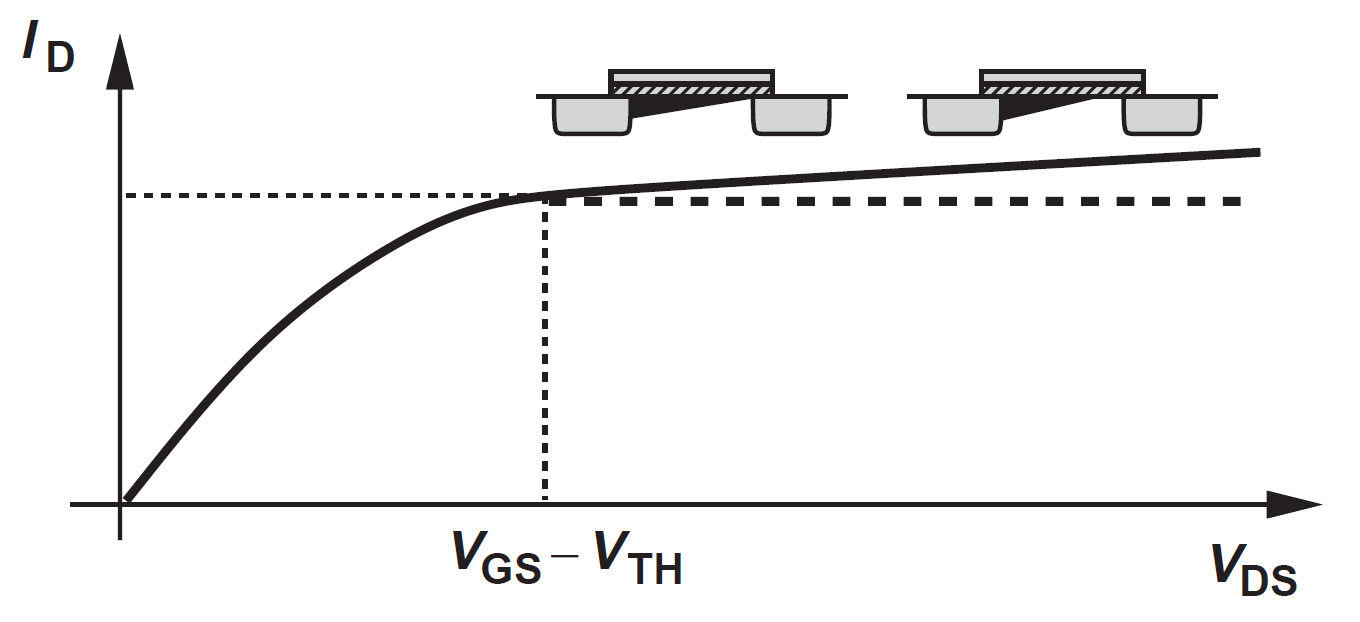
\includegraphics[width=0.7\textwidth]{figuras/modulacion_largo_canal_1.png}
\end{figure}

	\begin{tcolorbox}
		\[ I_D = \dfrac{K'}{2}\cdot\dfrac{W}{L} (V_{GS}-V_{TH})^2(1+\lambda V_{DS}) \]
	\end{tcolorbox}
	$\lambda$: coeficiente de modulación de canal [V\textsuperscript{-1}]
    
\end{frame}


\begin{frame}{Resistencia de salida}

Se define la resistencia de salida como la pendiente de la curva de salida:

\[ r_o = \left.\left[\dfrac{\partial I_{D}}{\partial V_{DS}}\right]^{-1}\right|_{V_{GSQ}} \]

\[ \dfrac{1}{r_o} = \dfrac{d}{dV_{DS}} \left\{ \dfrac{1}{2} \mu_n C_{ox}' \dfrac{W}{L} \left( V_{GS} - V_{TH} \right)^2 \left( 1 + \lambda V_{DS} \right) \right\} \]

\[ \dfrac{1}{r_o} = \lambda I_D \]

\[ \Rightarrow r_o = \dfrac{1}{\lambda I_D} \]

\end{frame}


\section{Ejemplo 1}
\begin{frame}{Ejemplo 1: Modulación de longitud de canal}

Determine la corriente $I_D$ y las tensiones $V_{GS}$, $V_{DS}$, considerando $\lambda \neq 0$.

\begin{columns}

\begin{column}{0.3\textwidth}

\begin{figure}[H]
    \centering
    \begin{circuitikz}[arrowmos]
        \draw (0,0) node[nmos](M1){$M_1$};
        \draw (-2,2) to[R,l=$R_1$] (-2,0);
        \draw (-2,0) to[R,l=$R_2$] (-2,-2);
        \draw (-2,-2) node[ground]{};
        \draw (-2,2) node[vdd]{$V_{DD}$};
        \draw (-2,0) to[short] (M1.gate);
        \draw (0,2) to[R,l=$R_D$] (M1.drain);
        \draw (0,2) node[vdd]{$V_{DD}$};
        \draw (M1.source) to[short] (0,-2);
        %\draw (M1.source) to[R,l=$R_S$] (0,-2);
        \draw (0,-2) node[ground]{};
    \end{circuitikz}
\end{figure}

\end{column}

\begin{column}{0.35\textwidth}

\centering
\textbf{Parámetros de la tecnología}
\[ \mu_n C_{ox}' = 100\ \mu A/V^2 \]
\[ \dfrac{W}{L} = \dfrac{10}{0.18} \]
\[ V_{TH} = 0.5\ V \]
\[ \lambda = 0.1\ V^{-1} \]

\end{column}

\begin{column}{0.35\textwidth}

\centering
\textbf{Parámetros del circuito}
\[ V_{DD} = 3.3\ V \]
\[ R_1 = 22\ k\Omega \]
\[ R_2 = 10\ k\Omega \]
\[ R_D = 1\ k\Omega \]
\end{column}

\end{columns}

\end{frame}


\begin{frame}{Solución 1: Modulación de longitud de canal}

\begin{columns}

\begin{column}{0.3\textwidth}

\begin{figure}[H]
    \centering
    \begin{circuitikz}[arrowmos]
        \draw (0,0) node[nmos](M1){$M_1$};
        \draw (-2,2) to[R,l=$R_1$] (-2,0);
        \draw (-2,0) to[R,l=$R_2$] (-2,-2);
        \draw (-2,-2) node[ground]{};
        \draw (-2,2) node[vdd]{$V_{DD}$};
        \draw (-2,0) to[short] (M1.gate);
        \draw (0,2) to[R,l=$R_D$] (M1.drain);
        \draw (0,2) node[vdd]{$V_{DD}$};
        \draw (M1.source) to[short] (0,-2);
        %\draw (M1.source) to[R,l=$R_S$] (0,-2);
        \draw (0,-2) node[ground]{};
    \end{circuitikz}
\end{figure}

\end{column}

\begin{column}{0.7\textwidth}

\[ I_D = \dfrac{1}{2} \mu_n C_{ox}' \dfrac{W}{L} (V_{GS} - V_{TH})^2 (1 + \lambda V_{DS}) \]
\[ V_{GS} = \dfrac{V_{DD} \cdot R_2}{R_1 + R_2} \]
\[ V_{DS} = V_{DD} - I_D R_D \]

Combinando las ecuaciones anteriores:
\[ I_D = \dfrac{1}{2} \mu_n C_{ox}' \dfrac{W}{L} \left( \dfrac{V_{DD} \cdot R_2}{R_1 + R_2} - V_{TH} \right)^2 \left(1 + \lambda (V_{DD} - I_D R_D) \right) \]

\begin{itemize}
    \item Esta es una ecuación lineal para $I_D$.
    \item Se puede resolver a mano despejando $I_D$.
\end{itemize}

\end{column}

\end{columns}

\end{frame}


\begin{frame}{Solución 1: Modulación de longitud de canal}

Con los valores numéricos del problema:
\[ I_D = \dfrac{1}{2} (100\ \mu A/V^2) \dfrac{10}{0.18} \left( \dfrac{3.3\ V \cdot 10\ k\Omega}{22\ k\Omega + 10\ k\Omega} - 0.5\ V \right)^2 \left(1 + (0.1\ V^{-1}) (3.3\ V - I_D \cdot 1\ k\Omega) \right) \]

\begin{itemize}
    \item Trabajo en clase: encuentre la solución de la ecuación.
\end{itemize}


\vspace{5mm}
\textbf{Respuestas}

Ecuación: $0.00104267 - 1.07840x = 0$

Solución: [$0.000966871$]

\end{frame}


\begin{frame}{Solución 1: Modulación de longitud de canal}

\end{frame}


\section{Ejemplo 2}
\begin{frame}{Ejemplo 2: Modulación de longitud de canal con RS}

Determine la corriente $I_D$ y las tensiones $V_{GS}$, $V_{DS}$, considerando $\lambda \neq 0$.

\begin{columns}

\begin{column}{0.3\textwidth}

\begin{figure}[H]
    \centering
    \begin{circuitikz}[arrowmos]
        \draw (0,0) node[nmos](M1){$M_1$};
        \draw (-2,2) to[R,l=$R_1$] (-2,0);
        \draw (-2,0) to[R,l=$R_2$] (-2,-2);
        \draw (-2,-2) node[ground]{};
        \draw (-2,2) node[vdd]{$V_{DD}$};
        \draw (-2,0) to[short] (M1.gate);
        \draw (0,2) to[R,l=$R_D$] (M1.drain);
        \draw (0,2) node[vdd]{$V_{DD}$};
        %\draw (M1.source) to[short] (0,-2);
        \draw (M1.source) to[R,l=$R_S$] (0,-2);
        \draw (0,-2) node[ground]{};
    \end{circuitikz}
\end{figure}

\end{column}

\begin{column}{0.35\textwidth}

\centering
\textbf{Parámetros de la tecnología}
\[ \mu_n C_{ox}' = 100\ \mu A/V^2 \]
\[ \dfrac{W}{L} = \dfrac{10}{0.18} \]
\[ V_{TH} = 0.5\ V \]
\[ \lambda = 0.1\ V^{-1} \]

\end{column}

\begin{column}{0.35\textwidth}

\centering
\textbf{Parámetros del circuito}
\[ V_{DD} = 3.3\ V \]
\[ R_1 = 22\ k\Omega \]
\[ R_2 = 10\ k\Omega \]
\[ R_D = 1\ k\Omega \]
\[ R_S = 220\ \Omega \]
\end{column}

\end{columns}

\end{frame}


\begin{frame}{Solución 2: Modulación de longitud de canal con RS}

\[ I_D = \dfrac{1}{2} \mu_n C_{ox}' \dfrac{W}{L} \left( \dfrac{V_{DD} \cdot R_2}{R_1 + R_2} - I_D R_S - V_{TH} \right)^2 \left(1 + \lambda (V_{DD} - I_D R_D - I_D R_S) \right) \]

\begin{itemize}
    \item Esta es una ecuación cúbica para $I_D$.
    \item Una opción es desarrollar algebraicamente hasta encontrar una expresión de la forma $ax^3 + bx^2 + cx + d = 0$.
    \item La otra opción es utilizar el método SHIFT+SOLVE con distintos valores iniciales. El problema es que dos de las soluciones son complejas.
    \vspace{5mm}
    \item Trabajo en clase: encuentre las tres soluciones de la ecuación.
\end{itemize}

\vspace{5mm}
\textbf{Respuestas}

Ecuación: $-16402.2x^3 + 258.026x^2 - 1.95922x + 0.00104267 = 0$

Soluciones: [$0.000574$, $0.007579 - 0.007302i$, $0.007579 + 0.007302i$]


\end{frame}


\begin{frame}{Solución 2: Modulación de longitud de canal con RS}

\end{frame}




\section{Referencias}
\begin{frame}{Lecturas recomendadas}

\begin{itemize}
    \item Razavi, B. (2013). Fundamentals of microelectronics. Chapter 6: Physics of MOS transistors, 2nd ed., pp. 288-290, Wiley.
\end{itemize}

\end{frame}


\end{document}
